\documentclass[12pt]{article}
\usepackage{ceai}
\graphicspath{{../figs/}}

\begin{document}
\doublespacing	

\title{CE 488/5588: Applied AI for Engineering\\ \large Topic 13: Deep Neural Networks --- Foundations \& Architectures}
\author{}
\date{}
\maketitle

\begin{ch-box}
This chapter marks a transition in our course. Topics 1--12 covered classical machine learning: regression, classification, SVMs, Bayesian methods, clustering, and dimensionality reduction. These are data-driven, small-to-medium-scale models that function as reusable, well-characterized operators. Starting here, we enter the post-2020 era: deep neural networks that learn hierarchical representations, foundation models trained on web-scale corpora, and generative systems that create rather than classify. The question we begin with is not ``what'' but ``why now?''---neural networks have existed since the 1980s. What changed?
\end{ch-box}

\section{Overview: Why Deep Learning Works Now}

Neural networks are not new. The perceptron was introduced in 1958, backpropagation was formalized in the 1980s, and multi-layer perceptrons (MLPs) were covered earlier in this course (Topic 3). Yet for decades, deep networks were widely regarded as impractical. They were difficult to train, prone to overfitting, and computationally expensive. The prevailing view was that shallow models with careful feature engineering---SVMs, random forests, logistic regression---were the tools of choice for real-world problems.

Then, in 2012, a deep convolutional neural network called AlexNet won the ImageNet Large Scale Visual Recognition Challenge by a dramatic margin, reducing the top-5 error rate from 26\% to 15\%. Since then, deep learning has dominated every major benchmark in vision, language, speech, and beyond. What changed?

Three factors converged:

\begin{itemize}
    \item \textbf{Data.} The internet made available massive labeled datasets---millions of images, billions of text tokens---far beyond what earlier researchers could access. Deep networks are data-hungry; they need large datasets to realize their representational capacity.
    
    \item \textbf{Compute.} Graphics Processing Units (GPUs), originally designed for rendering graphics, turned out to be ideal for the matrix multiplications at the heart of neural network training. Parallel compute power increased by orders of magnitude, making it feasible to train networks with millions---and later billions---of parameters.
    
    \item \textbf{Algorithmic advances.} This is the focus of this chapter. A series of seemingly modest algorithmic improvements---better activation functions, smarter initialization, normalization techniques, and adaptive optimizers---collectively solved the practical barriers that had prevented deep networks from training effectively.
\end{itemize}

The third factor---the algorithmic breakthroughs---is what we explore first. Understanding \textit{why} deep networks can now be trained is essential for any engineer who will use, evaluate, or build upon them.

\section*{Learning Objectives}
After completing this chapter, you should be able to:
\begin{itemize}
    \item Explain the key algorithmic advances that made deep neural networks trainable: ReLU activation, weight initialization, batch normalization, and adaptive optimization (Adam).
    \item Describe the vanishing gradient problem and how modern activation functions address it.
    \item Explain the convolution operation and why CNNs are effective for spatial data (images, grids).
    \item Describe the self-attention mechanism and why Transformers replaced RNNs for sequence modeling.
    \item Explain the intuition behind diffusion models as a generative approach.
    \item Compare CNNs, Transformers, and diffusion models in terms of their strengths, weaknesses, and typical applications in engineering.
\end{itemize}

\section{The Numerical Secrets of Training Deep Networks}

To understand why deep networks were historically difficult to train, we must examine what happens during backpropagation---the algorithm that computes gradients and updates weights.

\subsection{The Vanishing Gradient Problem}

Recall from Topic 3 that backpropagation applies the chain rule to compute the gradient of the loss with respect to each weight in the network. For a network with $L$ layers, the gradient for an early layer involves a product of $L$ terms:

\begin{equation}
    \frac{\partial \mathcal{L}}{\partial \mathbf{W}^{(1)}} = \frac{\partial \mathcal{L}}{\partial \mathbf{a}^{(L)}} \cdot \frac{\partial \mathbf{a}^{(L)}}{\partial \mathbf{a}^{(L-1)}} \cdots \frac{\partial \mathbf{a}^{(2)}}{\partial \mathbf{a}^{(1)}} \cdot \frac{\partial \mathbf{a}^{(1)}}{\partial \mathbf{W}^{(1)}},
    \label{t13eq:chain}
\end{equation}

where $\mathbf{a}^{(\ell)}$ denotes the activation at layer $\ell$. Each term $\partial \mathbf{a}^{(\ell+1)} / \partial \mathbf{a}^{(\ell)}$ involves the derivative of the activation function. If these derivatives are consistently less than 1, the product decays \textit{exponentially} with depth.

Consider the sigmoid function $\sigma(x) = 1 / (1 + e^{-x})$, whose derivative is $\sigma'(x) = \sigma(x)[1 - \sigma(x)]$. The maximum value of this derivative is $0.25$ (at $x = 0$). For a 10-layer network, even in the best case, the gradient shrinks by a factor of $0.25^{10} \approx 10^{-6}$. Early layers receive essentially no gradient signal---they stop learning.

This is the \textbf{vanishing gradient problem}. It explains why pre-2010 neural networks were typically limited to 2--3 hidden layers. The converse problem---\textbf{exploding gradients}---occurs when derivatives exceed 1, causing gradients to grow exponentially and destabilize training.

\begin{figure}[ht]
    \centering
    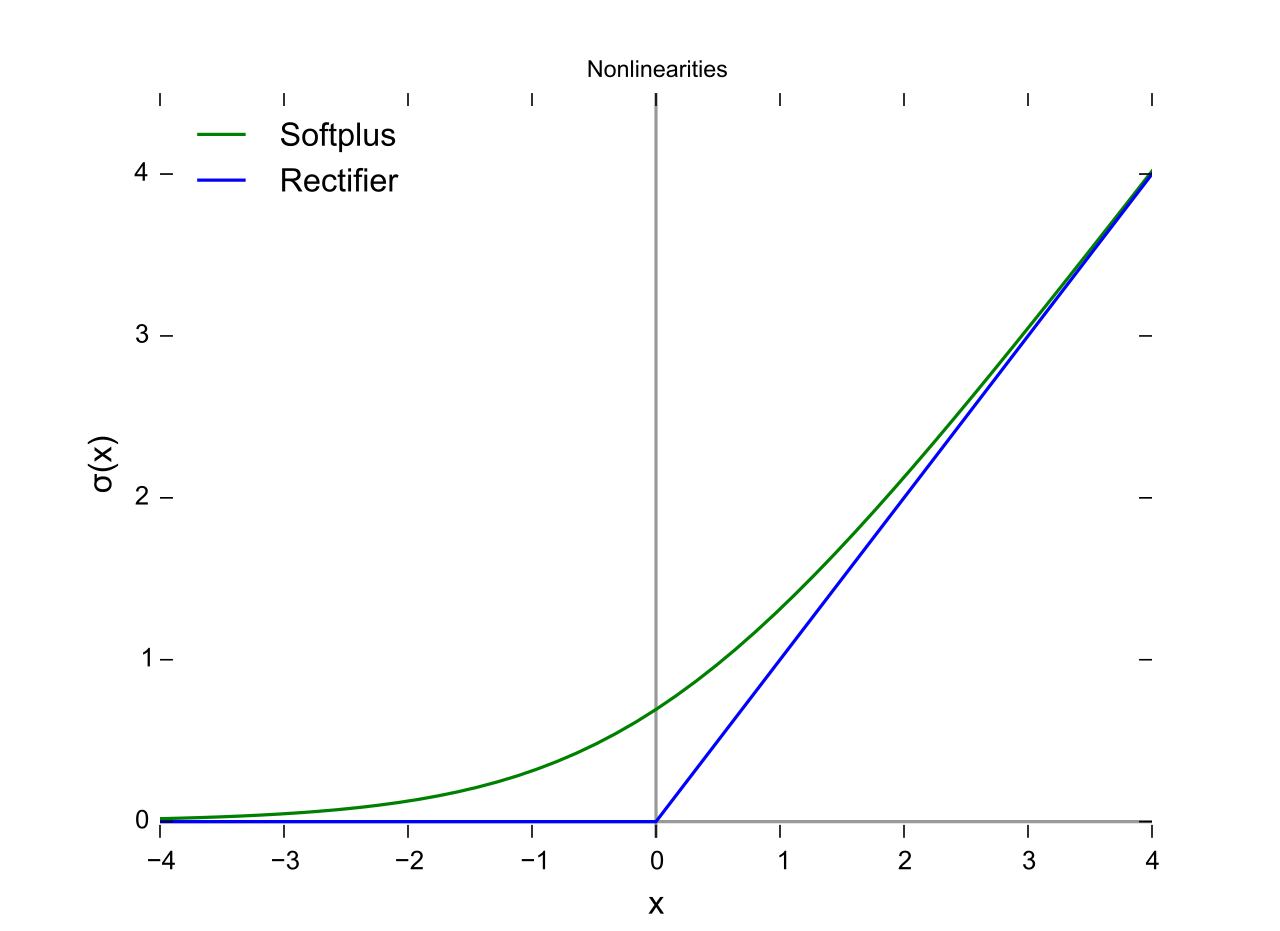
\includegraphics[width=0.55\textwidth]{Topic13fig01.png}
    \caption{Comparison of activation functions: sigmoid, tanh, and ReLU. Note that ReLU has a constant gradient of 1 for positive inputs, avoiding the vanishing gradient problem. \footnotemark}
    \label{t13fig:activations}
\end{figure}

\footnotetext{Figure adapted from educational resources on activation functions. See \url{https://en.wikipedia.org/wiki/Rectifier_(neural_networks)}.}

\subsection{ReLU and Modern Activation Functions}

The \textbf{Rectified Linear Unit} (ReLU) is defined simply as:

\begin{equation}
    \text{ReLU}(x) = \max(0, x).
    \label{t13eq:relu}
\end{equation}

Its derivative is:

\begin{equation}
    \text{ReLU}'(x) = \begin{cases} 
        1 & \text{if } x > 0, \\
        0 & \text{if } x \leq 0.
    \end{cases}
    \label{t13eq:relu_deriv}
\end{equation}

This simple change has profound consequences. For positive inputs, the gradient is exactly 1---it does not shrink with depth. A chain of 10 ReLU derivatives, each equal to 1, remains 1. The vanishing gradient problem is largely eliminated for the active path through the network.

ReLU also has computational advantages: it requires no exponentials (unlike sigmoid or tanh), making it significantly faster to compute on GPUs.

Variants address ReLU's one weakness---the ``dying ReLU'' problem, where neurons with consistently negative inputs output zero and stop learning:

\begin{itemize}
    \item \textbf{Leaky ReLU}: $\text{LeakyReLU}(x) = \max(\alpha x, x)$ with small $\alpha \approx 0.01$, allowing a small gradient for negative inputs.
    \item \textbf{GELU} (Gaussian Error Linear Unit): $\text{GELU}(x) = x \cdot \Phi(x)$, where $\Phi$ is the standard Gaussian CDF. This smooth, non-monotonic function is the default in modern Transformers (GPT, BERT).
\end{itemize}

\begin{alert-box}
\textbf{Key Insight:} ReLU's success is not about expressiveness---it is about \textit{gradient flow}. By maintaining a gradient of 1 for active neurons, ReLU allows error signals to propagate through dozens or hundreds of layers without exponential decay. This single change unlocked the training of deep architectures.
\end{alert-box}

\subsection{Weight Initialization}

Even with ReLU, a network can fail to train if weights are initialized poorly. If initial weights are too large, activations and gradients explode. If too small, they vanish. The goal is to keep the \textit{variance} of activations and gradients approximately constant across layers.

\textbf{Xavier/Glorot initialization} (for sigmoid/tanh):
\begin{equation}
    W_{ij} \sim \mathcal{N}\!\left(0,\; \frac{2}{n_{\text{in}} + n_{\text{out}}}\right),
    \label{t13eq:xavier}
\end{equation}
where $n_{\text{in}}$ and $n_{\text{out}}$ are the number of input and output connections.

\textbf{He initialization} (for ReLU):
\begin{equation}
    W_{ij} \sim \mathcal{N}\!\left(0,\; \frac{2}{n_{\text{in}}}\right).
    \label{t13eq:he}
\end{equation}

The factor of 2 in He initialization compensates for ReLU zeroing out negative inputs, which halves the variance. Proper initialization ensures that the network starts in a regime where gradients are neither vanishing nor exploding.

\subsection{Batch Normalization}

Even with good initialization, the distribution of activations at each layer shifts during training as upstream weights update. This phenomenon, called \textbf{internal covariate shift}, forces each layer to continuously adapt to a moving target, slowing convergence.

\textbf{Batch Normalization} (Ioffe \& Szegedy, 2015) addresses this by normalizing the activations of each layer across the mini-batch:

\begin{equation}
    \hat{x}_i = \frac{x_i - \mu_B}{\sqrt{\sigma_B^2 + \epsilon}}, \qquad
    y_i = \gamma \hat{x}_i + \beta,
    \label{t13eq:batchnorm}
\end{equation}

where $\mu_B$ and $\sigma_B^2$ are the mean and variance computed over the current mini-batch, $\epsilon$ is a small constant for numerical stability, and $\gamma, \beta$ are learnable parameters that allow the network to undo the normalization if beneficial.

Batch normalization has several effects:
\begin{itemize}
    \item Stabilizes training, allowing higher learning rates
    \item Acts as a mild regularizer (noise from mini-batch statistics)
    \item Reduces sensitivity to initialization
    \item Accelerates convergence
\end{itemize}

\subsection{Adaptive Optimization: From SGD to Adam}

Standard \textbf{Stochastic Gradient Descent} (SGD) updates weights as:
\begin{equation}
    \mathbf{w}_{t+1} = \mathbf{w}_t - \eta \nabla_{\mathbf{w}} \mathcal{L},
    \label{t13eq:sgd}
\end{equation}
where $\eta$ is a fixed learning rate. Choosing $\eta$ is delicate: too small, training is slow; too large, it diverges.

\textbf{Momentum} accumulates a velocity vector:
\begin{equation}
    \mathbf{v}_t = \beta \mathbf{v}_{t-1} + (1 - \beta) \nabla_{\mathbf{w}} \mathcal{L}, \qquad
    \mathbf{w}_{t+1} = \mathbf{w}_t - \eta \mathbf{v}_t,
    \label{t13eq:momentum}
\end{equation}
which smooths oscillations and accelerates progress in consistent gradient directions.

\textbf{Adam} (Adaptive Moment Estimation, Kingma \& Ba, 2015) combines momentum with per-parameter adaptive learning rates:
\begin{equation}
    m_t = \beta_1 m_{t-1} + (1 - \beta_1) g_t, \qquad
    v_t = \beta_2 v_{t-1} + (1 - \beta_2) g_t^2,
    \label{t13eq:adam}
\end{equation}
\begin{equation}
    \hat{m}_t = \frac{m_t}{1 - \beta_1^t}, \qquad
    \hat{v}_t = \frac{v_t}{1 - \beta_2^t}, \qquad
    \mathbf{w}_{t+1} = \mathbf{w}_t - \frac{\eta}{\sqrt{\hat{v}_t} + \epsilon} \hat{m}_t,
    \label{t13eq:adam_update}
\end{equation}
where $g_t = \nabla_{\mathbf{w}} \mathcal{L}$ is the gradient at step $t$. Adam maintains an exponentially weighted average of both the gradient ($m_t$, first moment) and the squared gradient ($v_t$, second moment), effectively giving each parameter its own adaptive learning rate.

\begin{alert-box}
\textbf{Summary of the Numerical Secrets:} The combination of ReLU (gradient flow), He initialization (starting right), batch normalization (stability), and Adam (adaptive learning rates) transformed deep networks from fragile, hard-to-train curiosities into robust, scalable systems. These are the algorithmic foundations that, together with data and compute, enabled the deep learning revolution.
\end{alert-box}

\section{Convolutional Neural Networks (CNNs)}

\subsection{From Hand-Crafted to Learned Features}

Classical computer vision relied on hand-crafted feature extractors: Sobel edges, SIFT descriptors, HOG features. These were designed by human experts to capture specific visual patterns. The key insight of CNNs is that \textit{features can be learned from data}---and that the learned features are typically superior to hand-crafted ones.

\subsection{The Convolution Operation}

A convolution applies a small filter (or kernel) $\mathbf{K}$ across an input image $\mathbf{I}$ by sliding the filter pixel-by-pixel and computing the element-wise product:

\begin{equation}
    (\mathbf{I} * \mathbf{K})_{i,j} = \sum_m \sum_n \mathbf{I}_{i+m,\,j+n} \cdot \mathbf{K}_{m,n}.
    \label{t13eq:conv}
\end{equation}

The filter $\mathbf{K}$ is a set of \textit{learnable parameters}. During training, the network discovers which patterns to detect: early layers learn edges and textures, intermediate layers learn shapes and parts, and deeper layers learn complex object components.

\begin{figure}[ht]
    \centering
    \includegraphics[width=0.6\textwidth]{Topic13fig02.png}
    \caption{The convolution operation: a $3 \times 3$ filter slides across the input, computing element-wise products at each position. The filter weights are learned during training. \footnotemark}
    \label{t13fig:convolution}
\end{figure}

\footnotetext{Figure adapted from educational resources on convolutional neural networks. See \url{https://en.wikipedia.org/wiki/Convolutional_neural_network}.}

Key hyperparameters:
\begin{itemize}
    \item \textbf{Filter size}: typically $3 \times 3$ or $5 \times 5$. Smaller filters are preferred in modern architectures (more layers, fewer parameters per layer).
    \item \textbf{Stride}: the step size of the filter movement. Stride 1 processes every position; stride 2 skips every other position (downsampling).
    \item \textbf{Padding}: adding zeros around the input border to preserve spatial dimensions.
\end{itemize}

\subsection{Pooling}

\textbf{Pooling} reduces spatial dimensions while retaining the most important information. \textbf{Max pooling} takes the maximum value in a window (e.g., $2 \times 2$):

\begin{equation}
    \text{MaxPool}(\mathbf{X})_{i,j} = \max_{m,n \in \text{window}} \mathbf{X}_{i+m,\,j+n}.
    \label{t13eq:maxpool}
\end{equation}

Pooling provides translation invariance (small shifts in the input produce the same output) and reduces computational cost.

\subsection{CNN Architecture Evolution}

\begin{figure}[ht]
    \centering
    \includegraphics[width=0.65\textwidth]{Topic13fig03.png}
    \caption{Evolution of CNN architectures: from LeNet (1998) to ResNet (2015). Depth increased from 5 layers to 152+ layers, enabled by algorithmic advances. \footnotemark}
    \label{t13fig:cnn_evolution}
\end{figure}

\footnotetext{Figure adapted from educational resources on CNN architecture evolution. See \url{https://medium.com/@siderealcs/a-brief-history-of-cnns-and-their-variants-70a7107bf886}.}

\begin{itemize}
    \item \textbf{LeNet-5} (LeCun et al., 1998): 5 layers, used for handwritten digit recognition. The first successful CNN.
    \item \textbf{AlexNet} (Krizhevsky et al., 2012): 8 layers, ReLU activation, GPU training. Won ImageNet 2012 by a large margin---the ``big bang'' of deep learning.
    \item \textbf{VGG} (Simonyan \& Zisserman, 2014): 16--19 layers, uniform $3 \times 3$ filters throughout. Demonstrated that depth matters more than filter size.
    \item \textbf{ResNet} (He et al., 2015): 50--152+ layers with \textbf{skip connections} (residual blocks). The key innovation:
    \begin{equation}
        \mathbf{y} = \mathcal{F}(\mathbf{x}, \{\mathbf{W}\}) + \mathbf{x},
        \label{t13eq:residual}
    \end{equation}
    where $\mathcal{F}$ is the residual function to be learned. The identity shortcut $\mathbf{x}$ ensures that the gradient can flow directly through the network, enabling training of very deep architectures.
\end{itemize}

\begin{figure}[ht]
    \centering
    \includegraphics[width=0.45\textwidth]{Topic13fig04.png}
    \caption{Residual block: the skip connection (identity shortcut) adds the input $\mathbf{x}$ directly to the output of the transformation $\mathcal{F}(\mathbf{x})$, enabling gradient flow through very deep networks. \footnotemark}
    \label{t13fig:residual}
\end{figure}

\footnotetext{Figure adapted from the original ResNet paper (He et al., 2015). See \url{https://arxiv.org/abs/1512.03385}.}

\subsection{Why CNNs Work: Key Properties}

\begin{itemize}
    \item \textbf{Translation equivariance}: a feature detected in one location can be detected anywhere. The same filter applies across the entire image.
    \item \textbf{Parameter sharing}: a $3 \times 3$ filter has only 9 parameters regardless of image size. This is dramatically more efficient than fully-connected layers.
    \item \textbf{Hierarchical feature learning}: early layers detect simple patterns (edges, corners), intermediate layers detect shapes and textures, deeper layers detect object parts and whole objects.
\end{itemize}

\subsection{Engineering Applications of CNNs}

\begin{itemize}
    \item \textbf{Crack detection in concrete}: CNNs trained on images of concrete surfaces can classify cracks with accuracy comparable to human inspectors, enabling automated structural health monitoring.
    \item \textbf{Construction progress monitoring}: CNNs analyze daily site photos to track construction progress against BIM models, identifying delays and discrepancies.
    \item \textbf{Material classification}: CNNs classify soil types, aggregate quality, and corrosion levels from field images.
    \item \textbf{Satellite imagery analysis}: CNNs detect land-use changes, monitor deforestation, and assess disaster damage from aerial and satellite imagery.
\end{itemize}

\section{Transformers}

\subsection{From RNNs to Attention}

Before Transformers, sequence modeling was dominated by \textbf{Recurrent Neural Networks} (RNNs) and their improved variant, \textbf{Long Short-Term Memory} (LSTM) networks. These process sequences one element at a time, maintaining a hidden state that carries information forward:

\begin{equation}
    \mathbf{h}_t = f(\mathbf{h}_{t-1}, \mathbf{x}_t).
    \label{t13eq:rnn}
\end{equation}

RNNs have two fundamental limitations:
\begin{itemize}
    \item \textbf{Sequential computation}: each step depends on the previous one, preventing parallelization during training.
    \item \textbf{Long-range dependency problem}: even with LSTMs, information from distant positions degrades over many time steps.
\end{itemize}

The \textbf{Transformer} (Vaswani et al., 2017) eliminated recurrence entirely, replacing it with \textbf{self-attention}---a mechanism that allows every position in a sequence to directly attend to every other position.

\subsection{Self-Attention Mechanism}

Self-attention computes a weighted sum of all input representations, where the weights are determined by the relevance (attention) of each input to the current position.

For an input sequence represented as a matrix $\mathbf{X} \in \mathbb{R}^{T \times d}$ (where $T$ is the sequence length and $d$ is the embedding dimension), we compute three projections:

\begin{equation}
    \mathbf{Q} = \mathbf{X}\mathbf{W}^Q, \quad
    \mathbf{K} = \mathbf{X}\mathbf{W}^K, \quad
    \mathbf{V} = \mathbf{X}\mathbf{W}^V,
    \label{t13eq:qkv}
\end{equation}

where $\mathbf{W}^Q, \mathbf{W}^K, \mathbf{W}^V \in \mathbb{R}^{d \times d_k}$ are learnable weight matrices. These are called \textbf{queries}, \textbf{keys}, and \textbf{values}---an analogy from information retrieval systems.

The attention output is:

\begin{equation}
    \text{Attention}(\mathbf{Q}, \mathbf{K}, \mathbf{V}) = \text{softmax}\!\left(\frac{\mathbf{Q}\mathbf{K}^\top}{\sqrt{d_k}}\right)\mathbf{V}.
    \label{t13eq:attention}
\end{equation}

The dot product $\mathbf{Q}\mathbf{K}^\top$ measures how relevant each position is to every other position. The softmax converts these scores into a probability distribution (attention weights). The scaling factor $1/\sqrt{d_k}$ prevents the dot products from growing too large, which would push the softmax into regions with tiny gradients.

\begin{figure}[ht]
    \centering
    \includegraphics[width=0.55\textwidth]{Topic13fig05.png}
    \caption{Self-attention mechanism: each token attends to all other tokens in the sequence, with attention weights computed from query-key compatibility. \footnotemark}
    \label{t13fig:self_attention}
\end{figure}

\footnotetext{Figure adapted from ``Attention Is All You Need'' (Vaswani et al., 2017). See \url{https://arxiv.org/abs/1706.03761} and \url{https://commons.wikimedia.org/wiki/File:Transformer,_full_architecture.png}.}

\subsection{Multi-Head Attention}

Instead of computing attention once, the Transformer computes it $H$ times in parallel, each with different learned projections. The outputs are concatenated and linearly transformed:

\begin{equation}
    \text{MultiHead}(\mathbf{X}) = \text{Concat}(\text{head}_1, \dots, \text{head}_H)\mathbf{W}^O,
    \label{t13eq:multihead}
\end{equation}
\begin{equation}
    \text{head}_i = \text{Attention}(\mathbf{X}\mathbf{W}_i^Q, \mathbf{X}\mathbf{W}_i^K, \mathbf{X}\mathbf{W}_i^V).
    \label{t13eq:head}
\end{equation}

Each head learns to focus on different aspects of the input: one might attend to syntactic relationships, another to semantic similarity, another to positional proximity. This is analogous to using multiple filters in a CNN, each detecting different patterns.

\subsection{Positional Encoding}

Since the Transformer has no recurrence or convolution, it has no inherent notion of position or order. To inject sequence order, \textbf{positional encodings} are added to the input embeddings:

\begin{equation}
    \text{PE}_{(pos, 2i)} = \sin\!\left(\frac{pos}{10000^{2i/d}}\right), \qquad
    \text{PE}_{(pos, 2i+1)} = \cos\!\left(\frac{pos}{10000^{2i/d}}\right),
    \label{t13eq:positional}
\end{equation}

where $pos$ is the position and $i$ is the dimension index. These sinusoidal encodings allow the model to attend to relative positions, since for any fixed offset $k$, $\text{PE}_{pos+k}$ can be represented as a linear function of $\text{PE}_{pos}$.

\subsection{Transformer Architecture}

The full Transformer consists of stacked blocks, each containing:
\begin{enumerate}
    \item \textbf{Multi-head self-attention}: captures relationships between all positions.
    \item \textbf{Feedforward network}: a two-layer MLP applied independently to each position:
    \begin{equation}
        \text{FFN}(\mathbf{x}) = \mathbf{W}_2 \cdot \text{GELU}(\mathbf{W}_1 \mathbf{x} + \mathbf{b}_1) + \mathbf{b}_2.
        \label{t13eq:ffn}
    \end{equation}
    \item \textbf{Residual connections} and \textbf{layer normalization} around each sublayer.
\end{enumerate}

\begin{figure}[ht]
    \centering
    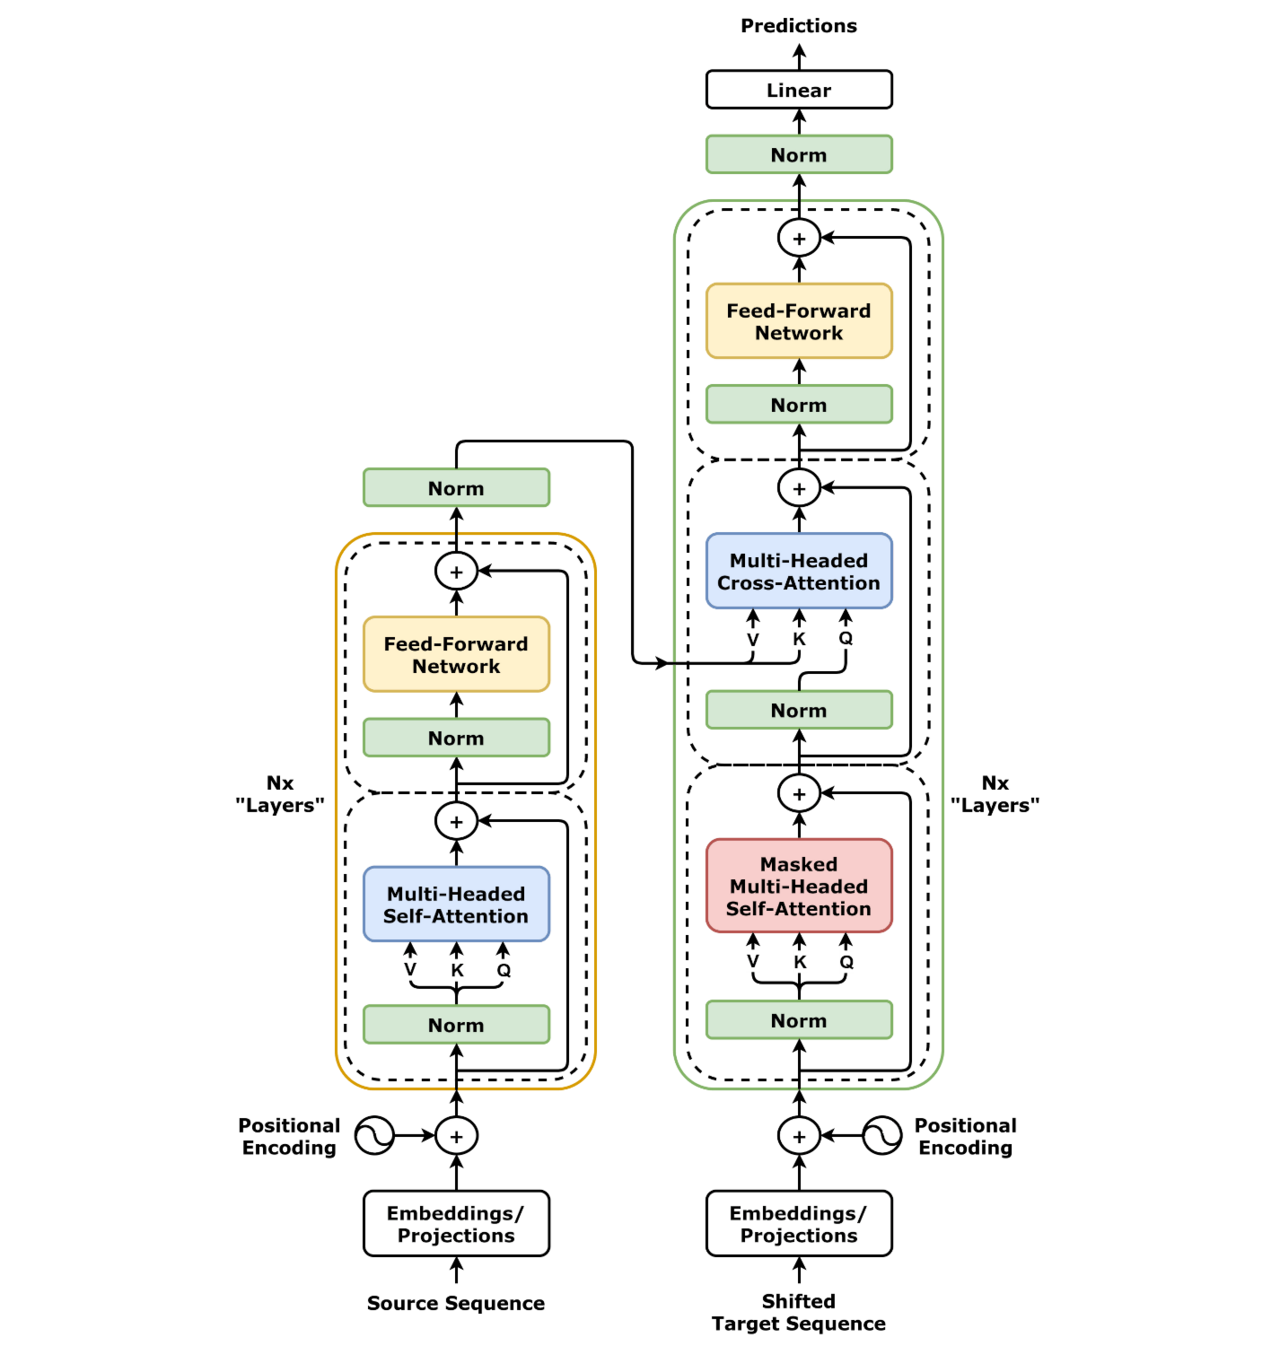
\includegraphics[width=0.45\textwidth]{Topic13fig06.png}
    \caption{The Transformer architecture (decoder-only, GPT-style): stacked blocks of self-attention and feedforward layers with residual connections and layer normalization. \footnotemark}
    \label{t13fig:transformer}
\end{figure}

\footnotetext{Figure adapted from ``Attention Is All You Need'' (Vaswani et al., 2017). See \url{https://arxiv.org/abs/1706.03761} and \url{https://commons.wikimedia.org/wiki/File:Attention_Is_All_You_Need_-_Encoder-decoder_Architecture.png}.}

There are three architectural variants:
\begin{itemize}
    \item \textbf{Encoder-only} (e.g., BERT): bidirectional attention, excellent for understanding tasks (classification, NER).
    \item \textbf{Decoder-only} (e.g., GPT): causal (masked) attention, each position attends only to previous positions. Used for generation.
    \item \textbf{Encoder-decoder} (e.g., T5, original Transformer): encoder processes input, decoder generates output with cross-attention. Used for translation, summarization.
\end{itemize}

\subsection{Why Transformers Replaced RNNs}

\begin{itemize}
    \item \textbf{Parallelization}: all positions are processed simultaneously, not sequentially. Training is dramatically faster.
    \item \textbf{Long-range dependencies}: every position directly attends to every other position, regardless of distance. No degradation over sequence length.
    \item \textbf{Scalability}: the architecture scales smoothly with data, compute, and model size---the foundation of modern LLMs.
\end{itemize}

The trade-off: self-attention has $O(T^2)$ complexity in sequence length, which becomes expensive for very long sequences. This is an active area of research (linear attention, sparse attention, state-space models).

\subsection{Engineering Applications of Transformers}

\begin{itemize}
    \item \textbf{Time-series forecasting}: Transformers model sensor data from structural health monitoring systems, predicting degradation trends and detecting anomalies.
    \item \textbf{Document understanding}: Transformers extract information from engineering reports, specifications, and contracts.
    \item \textbf{Code generation}: Transformers trained on code (e.g., Codex) assist engineers in writing analysis scripts, automating simulations, and generating documentation.
\end{itemize}

\section{Diffusion Models: An Introduction}

\subsection{The Intuition}

Diffusion models approach generation from a fundamentally different direction than GANs or VAEs. The core idea is elegantly simple:

\begin{enumerate}
    \item \textbf{Forward process}: gradually add Gaussian noise to a data sample over $T$ steps until it becomes pure noise.
    \item \textbf{Reverse process}: train a neural network to \textit{reverse} this noising process---to predict and remove the noise at each step, starting from pure noise and recovering data.
\end{enumerate}

Think of it as learning to unscramble an egg. The forward process scrambles; the reverse process unscrambles.

\begin{figure}[ht]
    \centering
    \includegraphics[width=0.7\textwidth]{Topic13fig07.png}
    \caption{Diffusion model: the forward process gradually adds noise to data until it becomes pure Gaussian noise. The reverse process, learned by a neural network, denoises step by step to generate new samples. \footnotemark}
    \label{t13fig:diffusion}
\end{figure}

\footnotetext{Figure adapted from educational resources on diffusion models. See \url{https://erdem.pl/2023/11/step-by-step-visual-introduction-to-diffusion-models} and \url{https://arxiv.org/abs/2406.08929}.}

\subsection{Forward Process}

The forward process is a fixed Markov chain that adds small amounts of Gaussian noise at each step $t = 1, \ldots, T$:

\begin{equation}
    q(\mathbf{x}_t \mid \mathbf{x}_{t-1}) = \mathcal{N}(\mathbf{x}_t; \sqrt{1 - \beta_t}\, \mathbf{x}_{t-1}, \beta_t \mathbf{I}),
    \label{t13eq:forward}
\end{equation}

where $\beta_t$ is a small noise schedule (e.g., $\beta_t$ increases from $10^{-4}$ to $0.02$ over $T = 1000$ steps). A remarkable property: we can sample $\mathbf{x}_t$ directly from $\mathbf{x}_0$ in one step:

\begin{equation}
    \mathbf{x}_t = \sqrt{\bar{\alpha}_t}\, \mathbf{x}_0 + \sqrt{1 - \bar{\alpha}_t}\, \boldsymbol{\epsilon}, \qquad
    \boldsymbol{\epsilon} \sim \mathcal{N}(\mathbf{0}, \mathbf{I}),
    \label{t13eq:forward_closed}
\end{equation}

where $\bar{\alpha}_t = \prod_{s=1}^t (1 - \beta_s)$.

\subsection{Reverse Process}

The reverse process is learned by a neural network $\boldsymbol{\epsilon}_\theta$ that predicts the noise added at each step:

\begin{equation}
    p_\theta(\mathbf{x}_{t-1} \mid \mathbf{x}_t) = \mathcal{N}(\mathbf{x}_{t-1}; \boldsymbol{\mu}_\theta(\mathbf{x}_t, t), \boldsymbol{\Sigma}_\theta(\mathbf{x}_t, t)).
    \label{t13eq:reverse}
\end{equation}

The training objective is remarkably simple: predict the noise $\boldsymbol{\epsilon}$ that was added to $\mathbf{x}_0$ to produce $\mathbf{x}_t$:

\begin{equation}
    \mathcal{L} = \mathbb{E}_{t, \mathbf{x}_0, \boldsymbol{\epsilon}} \left[ \left\| \boldsymbol{\epsilon} - \boldsymbol{\epsilon}_\theta(\mathbf{x}_t, t) \right\|^2 \right].
    \label{t13eq:diffusion_loss}
\end{equation}

This is just mean squared error between the true noise and the predicted noise. The network $\boldsymbol{\epsilon}_\theta$ is typically a U-Net architecture (an encoder-decoder CNN with skip connections).

\subsection{Why Diffusion Outperformed GANs}

\begin{itemize}
    \item \textbf{Training stability}: diffusion training is a simple regression problem (predict noise). GANs require balancing two networks in a minimax game, which is notoriously unstable.
    \item \textbf{Mode coverage}: diffusion models generate diverse samples covering the full data distribution. GANs often suffer from \textit{mode collapse}, generating only a subset of possible outputs.
    \item \textbf{Controllability}: by conditioning the noise prediction on text embeddings (via CLIP), diffusion models achieve text-to-image generation with remarkable fidelity (DALL-E, Stable Diffusion).
\end{itemize}

The trade-off: diffusion models require $T$ sequential denoising steps at generation time, making them slower than GANs (which generate in one forward pass). Recent work on consistency models and distillation has reduced this to 1--4 steps.

\subsection{Engineering Applications of Diffusion Models}

\begin{itemize}
    \item \textbf{Synthetic data generation}: diffusion models generate realistic structural images for training other models, especially for rare damage types where real data is scarce.
    \item \textbf{Design concept generation}: text-to-image diffusion models generate architectural renderings and design concepts from natural language descriptions.
    \item \textbf{Scenario visualization}: engineers can generate visualizations of structural scenarios (e.g., flood impact on infrastructure) for planning and communication.
\end{itemize}

\section{Summary: Comparing Architectures}

\begin{table}[ht]
    \centering
    \small
    \begin{tabulary}{\textwidth}{@{} L C C C @{}}
        \toprule
        \textbf{Property} & \textbf{CNNs} & \textbf{Transformers} & \textbf{Diffusion} \\
        \midrule
        \textbf{Primary use} & Vision (classification, detection) & Sequences (language, time-series) & Generation (images, audio) \\
        \textbf{Key operation} & Convolution + pooling & Self-attention & Iterative denoising \\
        \textbf{Inductive bias} & Translation equivariance, locality & Global relationships, position-agnostic & Gradual refinement \\
        \textbf{Training} & Supervised (labels) & Supervised / self-supervised & Self-supervised (noise prediction) \\
        \textbf{Parallelization} & High (within image) & High (within sequence) & Limited (sequential denoising) \\
        \textbf{Depth} & 50--200+ layers (ResNet) & 12--100+ blocks & U-Net (encoder-decoder) \\
        \bottomrule
    \end{tabulary}
    \caption{Comparison of the three major deep learning architectures covered in this chapter.}
    \label{t13tab:comparison}
\end{table}

Each architecture excels in its domain:
\begin{itemize}
    \item \textbf{CNNs} for spatial data (images, grids, spatial sensor data)---where local patterns and translation invariance matter.
    \item \textbf{Transformers} for sequential and relational data (text, time-series, graphs)---where long-range dependencies and global context matter.
    \item \textbf{Diffusion models} for generative tasks---where sample quality and diversity matter more than speed.
\end{itemize}

Modern systems often combine these: Vision Transformers (ViTs) apply self-attention to image patches; diffusion models use U-Net (CNN) backbones with Transformer attention layers; multimodal models integrate vision and language through cross-attention.

\section{Conclusion}

This chapter established the foundations of modern deep learning by answering the question: \textit{why now?} Neural networks existed for decades, but it was the convergence of algorithmic advances---ReLU activation, proper initialization, batch normalization, and adaptive optimization---that made training deep architectures practical and reliable.

We then examined the three architectures that define the post-2020 era. \textbf{CNNs} demonstrated that features can be learned rather than hand-crafted, achieving superhuman performance on visual recognition tasks. \textbf{Transformers} replaced recurrence with self-attention, enabling parallel training and modeling of arbitrarily long dependencies---the architecture behind every modern LLM. \textbf{Diffusion models} introduced a new paradigm for generation, learning to reverse a gradual noising process to produce high-quality, diverse samples.

These architectures are not competitors; they are complementary tools. CNNs excel at spatial understanding, Transformers at sequential and relational reasoning, and diffusion models at creative generation. Modern AI systems increasingly combine all three.

In the next chapter, we deepen our exploration of generative deep learning, examining GANs, VAEs, and diffusion models in greater detail---their architectures, training dynamics, trade-offs, and engineering applications. We will also explore how these generative models are used in practice for data augmentation, design generation, and synthetic scenario creation.

\end{document}
